% Options for packages loaded elsewhere
\PassOptionsToPackage{unicode}{hyperref}
\PassOptionsToPackage{hyphens}{url}
%
\documentclass[
]{book}
\usepackage{lmodern}
\usepackage{amssymb,amsmath}
\usepackage{ifxetex,ifluatex}
\ifnum 0\ifxetex 1\fi\ifluatex 1\fi=0 % if pdftex
  \usepackage[T1]{fontenc}
  \usepackage[utf8]{inputenc}
  \usepackage{textcomp} % provide euro and other symbols
\else % if luatex or xetex
  \usepackage{unicode-math}
  \defaultfontfeatures{Scale=MatchLowercase}
  \defaultfontfeatures[\rmfamily]{Ligatures=TeX,Scale=1}
\fi
% Use upquote if available, for straight quotes in verbatim environments
\IfFileExists{upquote.sty}{\usepackage{upquote}}{}
\IfFileExists{microtype.sty}{% use microtype if available
  \usepackage[]{microtype}
  \UseMicrotypeSet[protrusion]{basicmath} % disable protrusion for tt fonts
}{}
\makeatletter
\@ifundefined{KOMAClassName}{% if non-KOMA class
  \IfFileExists{parskip.sty}{%
    \usepackage{parskip}
  }{% else
    \setlength{\parindent}{0pt}
    \setlength{\parskip}{6pt plus 2pt minus 1pt}}
}{% if KOMA class
  \KOMAoptions{parskip=half}}
\makeatother
\usepackage{xcolor}
\IfFileExists{xurl.sty}{\usepackage{xurl}}{} % add URL line breaks if available
\IfFileExists{bookmark.sty}{\usepackage{bookmark}}{\usepackage{hyperref}}
\hypersetup{
  pdftitle={Matematika Bisnis},
  pdfauthor={Bakti Siregar, S.Si., M.Sc},
  hidelinks,
  pdfcreator={LaTeX via pandoc}}
\urlstyle{same} % disable monospaced font for URLs
\usepackage{longtable,booktabs}
% Correct order of tables after \paragraph or \subparagraph
\usepackage{etoolbox}
\makeatletter
\patchcmd\longtable{\par}{\if@noskipsec\mbox{}\fi\par}{}{}
\makeatother
% Allow footnotes in longtable head/foot
\IfFileExists{footnotehyper.sty}{\usepackage{footnotehyper}}{\usepackage{footnote}}
\makesavenoteenv{longtable}
\usepackage{graphicx,grffile}
\makeatletter
\def\maxwidth{\ifdim\Gin@nat@width>\linewidth\linewidth\else\Gin@nat@width\fi}
\def\maxheight{\ifdim\Gin@nat@height>\textheight\textheight\else\Gin@nat@height\fi}
\makeatother
% Scale images if necessary, so that they will not overflow the page
% margins by default, and it is still possible to overwrite the defaults
% using explicit options in \includegraphics[width, height, ...]{}
\setkeys{Gin}{width=\maxwidth,height=\maxheight,keepaspectratio}
% Set default figure placement to htbp
\makeatletter
\def\fps@figure{htbp}
\makeatother
\setlength{\emergencystretch}{3em} % prevent overfull lines
\providecommand{\tightlist}{%
  \setlength{\itemsep}{0pt}\setlength{\parskip}{0pt}}
\setcounter{secnumdepth}{5}
\usepackage{booktabs}
\usepackage{amsthm}
\makeatletter
\def\thm@space@setup{%
  \thm@preskip=8pt plus 2pt minus 4pt
  \thm@postskip=\thm@preskip
}
\makeatother
\usepackage[]{natbib}
\bibliographystyle{apalike}

\title{Matematika Bisnis}
\author{Bakti Siregar, S.Si., M.Sc}
\date{September 14, 2020}

\begin{document}
\maketitle

{
\setcounter{tocdepth}{1}
\tableofcontents
}
\hypertarget{selamat-datang}{%
\chapter*{Selamat Datang!}\label{selamat-datang}}
\addcontentsline{toc}{chapter}{Selamat Datang!}

\begin{center}\rule{0.5\linewidth}{0.5pt}\end{center}

\begin{center}
\includegraphics[width=0.5\linewidth]{images/cover} \end{center}

Program Studi Statistika
Fakultas Science, Technology, Engineering, and Mathematics (STEM)
Tangerang, Banten
Info: siregarbakti@gmail.com

\hypertarget{kata-pengantar}{%
\section*{Kata Pengantar}\label{kata-pengantar}}
\addcontentsline{toc}{section}{Kata Pengantar}

Buku ini dituliskan untuk mempermudah proses pembelajaran Matematika Bisnis di Universitas Matana. Materi dikemas secara khusus dalam bentuk e-book yang mudah dipahami dan dapat dibaca melalui PC maupun Tablet anda dimanapun-kapanpun dengan akses internet.

Adapun Materi yang akan dibahas dalam buku ini adalah sebagai berikut:

\begin{itemize}
\tightlist
\item
  Minggu 1 \textasciitilde{} Pengenalan Matematika Bisnis
\item
  Minggu 2 \textasciitilde{} Dasar Matematika Bisnis
\item
  Minggu 3 \textasciitilde{} Matematika Manajemen Bisnis
\item
  Minggu 4 \textasciitilde{} Sumber Daya Manusia dan Aplikasi Ekonomi
\item
  Minggu 5 \textasciitilde{} Dasar-dasar Pemasaran dan Akuntansi
\item
  Minggu 6 \textasciitilde{} Aplikasi Pemasaran
\item
  Minggu 7 \textasciitilde{} Aplikasi Akuntansi
\item
  Minggu 8 \textasciitilde{} Ujian Tengah Semester
\item
  Minggu 9 \textasciitilde{} Bunga Sederhana- Bekerja Dengan Pembayaran Tunggal dan Aplikasi
\item
  Minggu 10 \textasciitilde{} Bunga Majemuk- Bekerja Dengan Pembayaran Tunggal
\item
  Minggu 11 \textasciitilde{} Bunga Majemuk- Aplikasi yang Melibatkan Pembayaran Tunggal
\item
  Minggu 12 \textasciitilde{} Bunga Majemuk- Anuitas
\item
  Minggu 13 \textasciitilde{} Bunga Majemuk- Aplikasi Khusus Anuitas
\item
  Minggu 14 \textasciitilde{} Memahami Amortisasi dan Aplikasinya
\item
  Minggu 15 \textasciitilde{} Obligasi dan Dana Tenggelam
\item
  Minggu 16 \textasciitilde{} Ujian Akhir
\end{itemize}

\hypertarget{tentang-penulis}{%
\section*{Tentang Penulis}\label{tentang-penulis}}
\addcontentsline{toc}{section}{Tentang Penulis}

Bakti Siregar adalah lulusan Universitas Sumatera Utara (USU), Jurusan Matematika. Setelah meluluskan S1 nya di tahun 2013, langsung mendapatkan perkerjaan di PT. Asuransi Sinar Mas sebagai Underwriter Managament Trainee. Di tahun 2014 beranjak ke perusahaan Multifinance sebagai Credit Analyst. Tak lama berselang, Beliau memutuskan untuk melanjutkan studinya dan berhasil memperoleh gelar Masternya dengan beasiswa yang diperoleh dari National Sun Yat-sen University (NSYSU-Taiwan), Jurusan Matematika Terapan Sains Data (Data Science).

Selain menjadi seseorang yang berfrofesi sebagai Data Scientist, beliau juga menjadi dosen di Prodi Statistika Universitas Matana, Tengerang. Bakti Siregar secara spesifik berfokus untuk mengajar dan juga meneliti dibidang Matematika Bisnis, Statistika Bisnis, Ekonometrika, Analisis Runtun Waktu, Algoritma dan Struktur Data, Sistem Basis Data, Metodologi Penelitian, Kalkulus, Aljabar Linear, Metode Statistika, Komputasi Statistika, Optimisasi, dll. Dia adalah instruktur berdedikasi yang tertarik untuk membantu siswanya berhasil melalui pengajaran multi-media yang melibatkan PowerPoint, video, diskusi dalam kelas, bacaan perangkat lunak online (e-book), dan menyusun soal-soal latihan secara progresif untuk mempermudah mahasiswa/i dalam menyelesaikan tugas-tugasnya.

Bakti Siregar tinggal di Bekasi, Jawa barat, Indonesia, bersama adik laki-lakinya yang sedang menempuh perkuliahan di program studi Manajemen. Ketika dia tidak mengajar, dia suka berlibur di iklim Sejuk seperti Puncak, Bogor, dan Bandung bersama sanak saudaranya.

\begin{center}\rule{0.5\linewidth}{0.5pt}\end{center}

Bakti Siregar, S.Si., M.Sc
Email: \href{mailto:siregarbakti@gmail.com}{\nolinkurl{siregarbakti@gmail.com}} / \href{mailto:siregar.bakti@matanauniversity.ac.id}{\nolinkurl{siregar.bakti@matanauniversity.ac.id}}
Github: \url{https://github.com/Bakti-Siregar}
LinkedIn: \url{https://www.linkedin.com/in/bakti-siregar-15955480/}

\hypertarget{Pendahuluan}{%
\chapter{Pendahuluan}\label{Pendahuluan}}

\begin{center}\rule{0.5\linewidth}{0.5pt}\end{center}

Bab ini, sedang dalam proses penulisan. Akan segera update. Bagian ini hanya membahas mengenai kontrak kuliah, rencana pembelajaran, dan tinjauan penilaian yang dilakukan dosen pengampu.

\hypertarget{Dasar-Matematika-Bisnis}{%
\chapter{Dasar Matematika Bisnis}\label{Dasar-Matematika-Bisnis}}

\begin{center}\rule{0.5\linewidth}{0.5pt}\end{center}

Kemana anda bisa pergi dalam hidup dan tidak mengenal angka dan matematika? Bahkan saat anda sedang mencari tahu harga suatu produk (termasuk pengiriman) di Lazada, Tokopedia, Traveloka, dll. Begitupun saat mengatur pemasukan dan pengeluaran di rekening bank anda, dalam hal ini diperlukan keterampilan matematika sederhana dari pendidikan dasar dan hingga pendidikan menengah. Berikut ini diulas beberapa contoh sederhana mengenai penerapan matematika yang anda lakukan setiap hari:

\begin{itemize}
\tightlist
\item
  Di toko bahan makanan, anda seringkali membandingkan produk untuk menghitung nilai terbaik. Satu merek keripik kentang dijual seharga \(\$ 3,99\) untuk 300 g, sedangkan merek yang sama memuaskannya di sampingnya seharga \(\$ 3,49\) untuk 250 g. Mana yang menawarkan nilai lebih baik?
\item
  Jika anda adalah penggemar olahraga, anda tahu banyak statistik tentang pemain dan tim favorit anda. Banyak yang datang dalam bentuk persentase, seperti lemparan tiga poin untuk bintang NBA atau menyimpan persentase untuk penjaga gawang NHL. Apa sebenarnya arti persentase tersebut?
\item
  Banyak majikan membayar bonus. Mungkin di perusahaan anda, manajer mendapatkan bonus dua kali lebih besar daripada karyawan. Perusahaan anda memiliki lima manajer dan 25 karyawan. Jika mengumumkan bonus total \(\$ 35.000,\) berapa bagian anda sebagai karyawan?
\end{itemize}

Sadar atau tidak Matematika dan angka mengelilingi anda di dunia bisnis, termasuk saat anda harus membaca banyak laporan numerik, menafsirkan bagaimana angka-angka itu cocok, dan membuat laporan anda sendiri yang menunjukkan metrik seperti proyeksi penjualan dan laba. Diluar pekerjaan, anda juga harus mengelola pendapatan dan membayar tagihan anda. Ini adalah masalah matematika yang mungkin anda pecahkan setiap hari, memastikan bahwa uang yang mengalir keluar dari rekening bank anda tidak melebihi uang yang mengalir masuk. Untuk membeli bahan makanan, liburan, atau hiburan, dalam hal ini ada perlu untuk mempertimbangkan prioritas utama.

Bab ini mengulas tentang keterampilan matematika dasar yang menjadi acuan penting di bab-bab selanjutnya. Beberapa contoh akan dijelaskan secara rinci, sementara yang lain akan diseerahkan kepada anda untuk menyelesaikan bab ini secara mandiri. Bagaimanapun, bab ini penting dan harus digunakan untuk menguji kemampuan dasar anda. Olehkarena itu, pelajarilah bab ini dengan percaya diri, dan jika anda menemui kesulitan, pastikan anda menguasai konsep sebelum melanjutkan ke bab berikutnya.

\hypertarget{urutan-perhitungan}{%
\section{Urutan Perhitungan}\label{urutan-perhitungan}}

Andaikan baru saja anda memenangkan \(\$ 50.000\) dalam sebuah undian, Yeah\ldots{} Selamat untuk Anda! Tetapi sebelum dapat mengklaimnya, anda diminta untuk menjawab pertanyaan pengujian keterampilan matematika, dan tidak ada kalkulator yang diizinkan. Setelah anda menyerahkan tiket kemenangan ke agen penukaran, dia memberikan pertanyaan pengujian keterampilan terbatas waktu: 2 × 5 + 30 ÷ 5. Saat waktu dihitung mundur, anda pasti mempertimbangkan berbagai kemungkinan. Apakah jawabannya 8, 14, 16, atau sama sekali berbeda? Bukankah sangat buruk kehilangan \$ 50.000 karena anda tidak dapat menjawab pertanyaan itu! Jika anda menemukan solusinya adalah 16, anda berada di jalan yang benar. Sebaliknya jika anda memperoleh jawaban berbeda, inilah saat yang tepat untuk meninjau ulang cara anda melakukan perhitungan.

Dalam buku ini akan diperkenalkan operasi perhitungan matematika dengan menggunakan EXcel yang mungkin saja memiliki kesamaan dengan beberapa Kalkulator atau Applikasi. Operator yang anda gunakan dalam Excel adalah factor yang paling krusial saat melakukan penghitungan yang ingin Anda lakukan pada elemen suatu rumus. Excel mengikuti aturan matematika umum untuk penghitungan, yaitu Tanda Kurung (Parentheses), Eksponen (Exponents), Perkalian dan Pembagian (Multiplication and Division), serta Penambahan dan Pengurangan (Addition and Subtraction). Perlu dicatat bahwa penggunaan tanda kurung memungkinkan anda mengubah urutan penghitungan tersebut.

\hypertarget{operator-aritmetika}{%
\section{Operator Aritmetika}\label{operator-aritmetika}}

Untuk melakukan operasi matematika dasar, seperti penambahan, pengurangan, perkalian, atau pembagian; menggabungkan angka; dan menghasilkan nilai numerik, anda dapat menggunakan operator aritmetika berikut ini dalam Excel.

\begin{figure}

{\centering 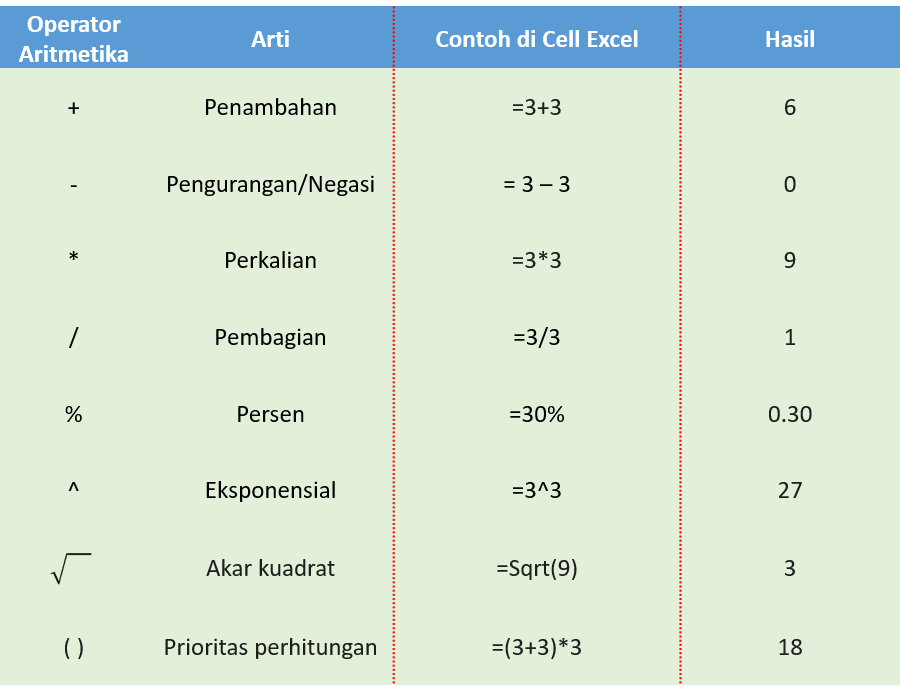
\includegraphics[width=0.75\linewidth]{images/aritmatika} 

}

\caption{Operator Aritmetika}\label{fig:aritmatika}
\end{figure}

\textbf{Catatan:} () atau {[}{]} atau \{\} Secara berurutan, ini dikenal sebagai tanda kurung bulat, persegi, dan keriting.

\hypertarget{operator-perbandingan}{%
\section{Operator Perbandingan}\label{operator-perbandingan}}

Saat dua nilai dibandingkan dengan menggunakan operator ini, hasilnya adalah nilai logika---TRUE atau FALSE. Anda juga dapat membandingkan dua nilai dengan operator berikut dalam Excel.

\begin{figure}

{\centering 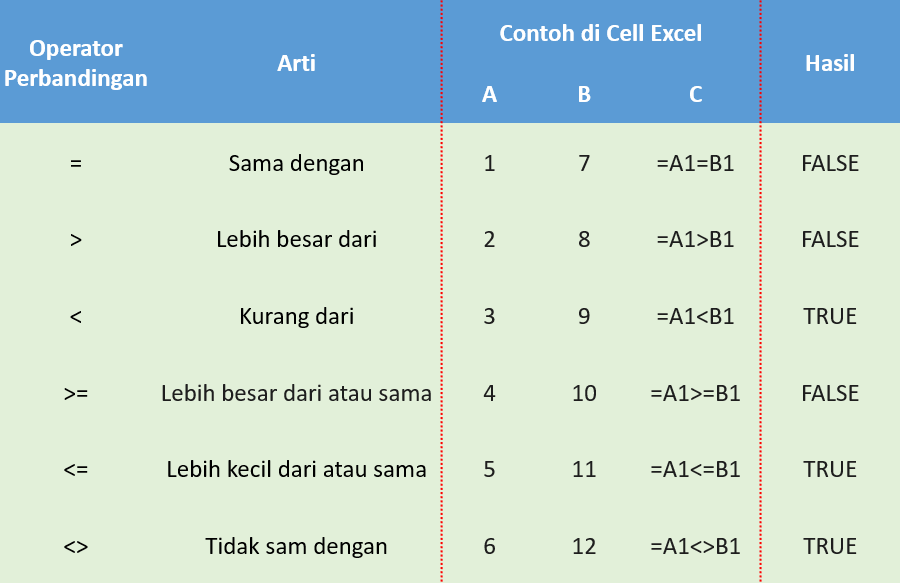
\includegraphics[width=0.75\linewidth]{images/perbandingan} 

}

\caption{Operator Perbandingan}\label{fig:perbandingan}
\end{figure}

\hypertarget{operator-referensi}{%
\section{Operator Referensi}\label{operator-referensi}}

Pada bagian ini ada diharapakan untuk dapat menggunakan penggabungan rentang sel untuk perhitungan dengan operator dalam Excel.

\begin{figure}

{\centering 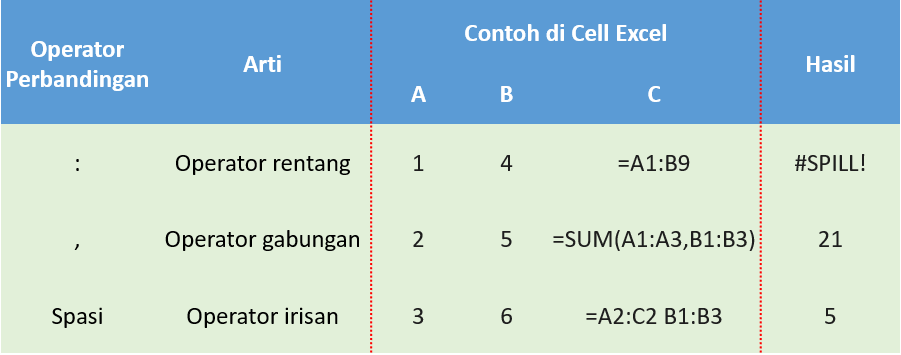
\includegraphics[width=0.75\linewidth]{images/referensi} 

}

\caption{Operator Referensi}\label{fig:referensi}
\end{figure}

\textbf{Catatan:} Kesalahan \#SPILL dikembalikan saat rumus mengembalikan beberapa hasil, dan Excel tidak bisa mengembalikan hasil ke Cell. Operator rentang \texttt{:} ini tidak dapat berdiri sendiri.

\hypertarget{sistem-persamaan-linear}{%
\section{Sistem Persamaan Linear}\label{sistem-persamaan-linear}}

Sistem persamaan linear adalah persamaan-persamaan linear yang dikorelasikan untuk membentuk suatu sistem. Sistem persamaannya bisa terdiri dari satu variabel, dua variabel atau lebih. Dalam bahasan ini, kita hanya membahas sistem persamaan linear dengan dua dan tiga variabel.

\hypertarget{sistem-persamaan-linear-dua-variabel-spldv}{%
\subsection{Sistem Persamaan Linear Dua Variabel (SPLDV)}\label{sistem-persamaan-linear-dua-variabel-spldv}}

Sistem persamaan linear dua variabel adalah sistem persamaan linear yang terdiri dari dua persamaan dimana masing-masing persamaan memiliki dua variabel. Bentuk umum SPLDV dengan variabel x dan y:

Sebagai contoh ada dua persamaan linier yaitu

\begin{itemize}
\tightlist
\item
  \(y_1 = 10 -2x\) dan
\item
  \(y_2 = 2 + 2x\) ,
\end{itemize}

maka penyelesaian sistem persamaan linier tersebut adalah

\textbf{Langkah 1}, mencari nilai \(x:\)

\[
\begin{aligned}
y_1   &= y_2 \\
10-2x &= 2+2x\\
10-2x-2-2x &= 0 \\
-4x &= -8\\
x &= {8\over 4} \\
x &= 2 \\
\end{aligned}
\]

\textbf{Langkah 2}, mencari Nilai \(y,\)

diktehui nilai pertemuan pada \(x=2\), maka dimasukan dalam persamaan pertama yaitu

\[
\begin{aligned}
y &= 10-2x \\
y &= 10-(2 \times 2)
\end{aligned}
\]

Jadi nilai persamaan 1 dan 2 adalah \(x=2\) dan \(y=6\) atau pada koordinat (2,6). Jadi kesimpulanya adalah Tujuan dari sietem persamaan Linier adalah mencari nilai pertemuan antara dua persamaan garis lurus, yang dapat dicari gengan menggunakan metode Substitusi dan metode eliminasi.

Contoh juga juga dapat diselesaikan dengan menggunakan Excel. persamaan diatas dapat kita sederhanakan menjadi sistem persamaan linear berikut ini:

\begin{itemize}
\tightlist
\item
  \(2x + y = 10\)
\item
  \(-2x +y = 2\)
\end{itemize}

Dalam notasi matriks, ini dapat ditulis sebagai \(AX = B\)

\[ A=
\begin{bmatrix}
    2 & 1 &  \\
   -2 & 1 
\end{bmatrix}, 
\begin{bmatrix}
    x  \\
   y 
\end{bmatrix},
\begin{bmatrix}
    10  \\
   2 
\end{bmatrix}
\]

Jika \(A^{-1}\) (kebalikan dari matriks \(A\)) ada, kita dapat mengalikan kedua sisi dengan \(A^{-1}\) untuk mendapatkan \(X = A^{-1}B\). Untuk mengatasi sistem persamaan linear dengan Microsoft Excel, jalankan langkah-langkah yang terlampir pada \href{https://github.com/Bakti-Siregar/Matematika-Bisnis/raw/master/data/dasar-matematika-bisnis.xlsx}{file Exel ini}. Perlu dicatat bahwa dalam file ini juga terlampir Soal kasus 1.1 s/d kasus 1.6.

\hypertarget{latihan-1}{%
\section{Latihan 1}\label{latihan-1}}

\hypertarget{kasus-1.1}{%
\subsection*{Kasus 1.1}\label{kasus-1.1}}
\addcontentsline{toc}{subsection}{Kasus 1.1}

Andaikan diketahui harga menu Kopi Dari Hati di Toko A dan Toko B secara berturut-turut pada cell A dan B yang terlampir pada gambar \ref{fig:tabel1}, lakukan evaluasi operasi matematika dasar untuk melengkapi laporan tersebut.

\begin{figure}

{\centering 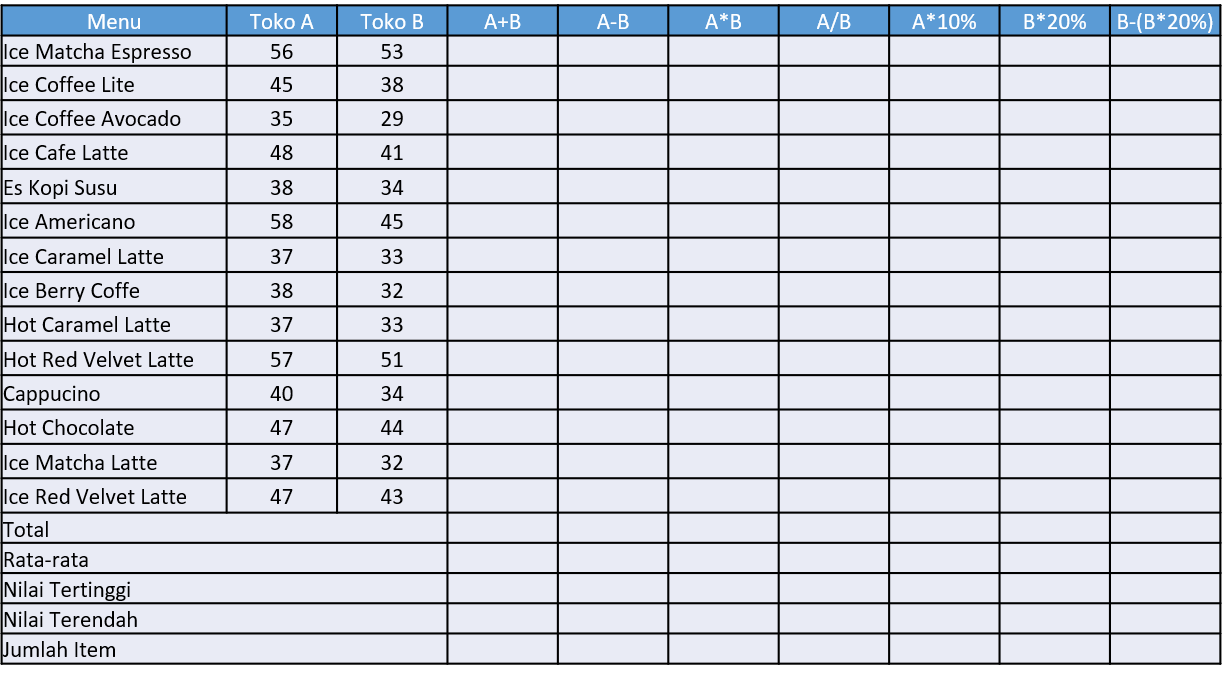
\includegraphics[width=1\linewidth]{images/tabel1} 

}

\caption{Harga Menu Toko A dan B}\label{fig:tabel1}
\end{figure}

\hypertarget{kasus-1.2}{%
\subsection*{Kasus 1.2}\label{kasus-1.2}}
\addcontentsline{toc}{subsection}{Kasus 1.2}

Diberikan daftar Karyawan PT. Kopi Dari Hati \textasciitilde{} Cabang Tangerang, September 2020, pada gambar \ref{fig:tabel2}. Pada bagian ini digunakan fungsi seperti SUM, MIN, AVERAGE, dan MAX.

\begin{figure}

{\centering 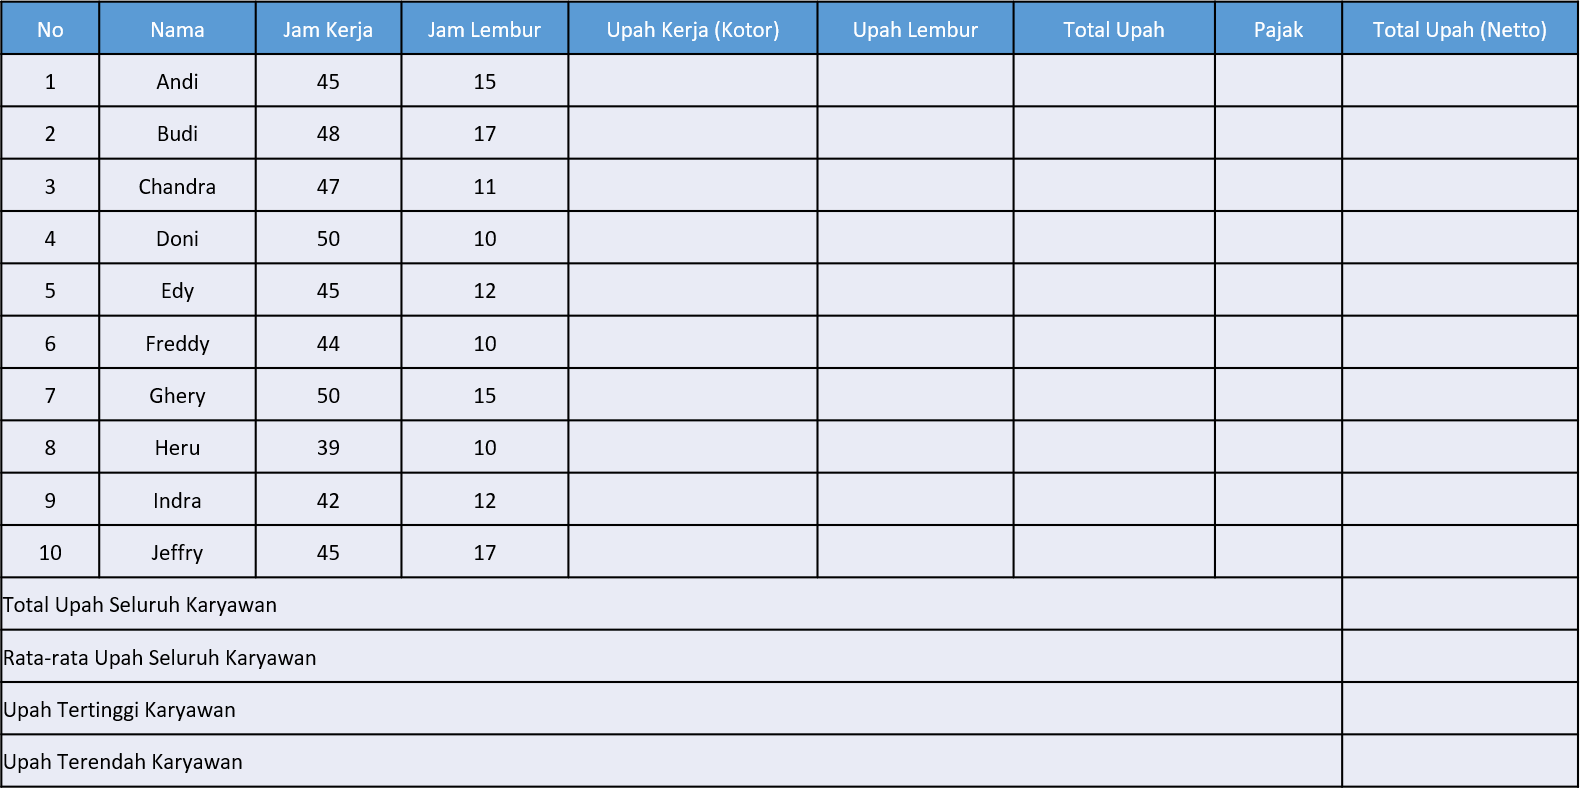
\includegraphics[width=1\linewidth]{images/tabel2} 

}

\caption{Daftar Karyawan}\label{fig:tabel2}
\end{figure}

\textbf{Keterangan:}

\begin{itemize}
\tightlist
\item
  Upah Kerja (Kotor) = Jam Kerja x 25000
\item
  Upah Lembur = Jam Lembur x 30000
\item
  Total Upah = Upah Kerja + Upah Lembur
\item
  Pajak = Total Upah x 5\%
\item
  Total Upah (Netto) = Total Upah -- Pajak
\end{itemize}

\hypertarget{kasus-1.3}{%
\subsection*{Kasus 1.3}\label{kasus-1.3}}
\addcontentsline{toc}{subsection}{Kasus 1.3}

Pada bagian ini anda diharapkan untuk mampu menerapkan Fungsi VLOOKUP untuk mengitung Harga Penjualan Kopi Dari Hati, lihat gambar \ref{fig:tabel3}.

\begin{figure}

{\centering 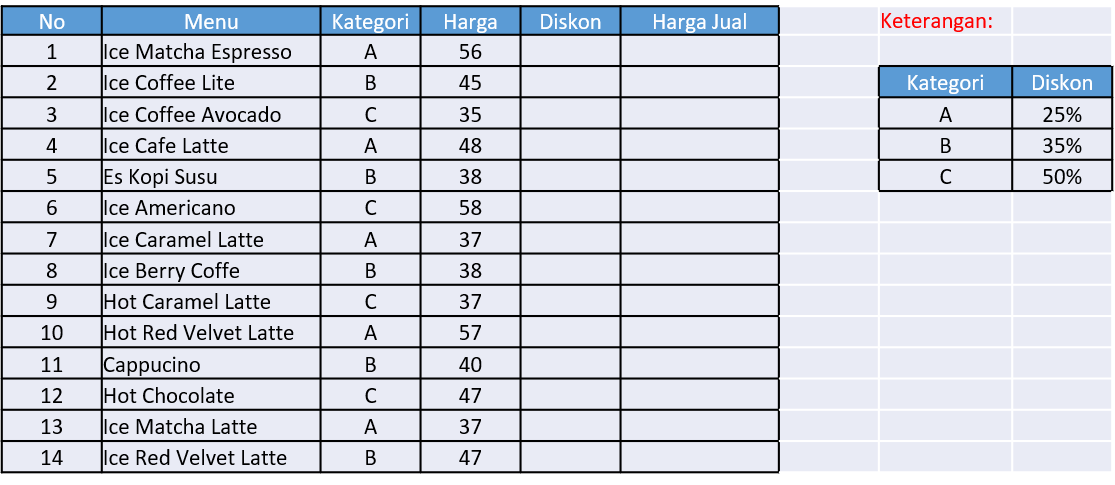
\includegraphics[width=1\linewidth]{images/tabel3} 

}

\caption{Harga Penjualan Kopi Dari Hati}\label{fig:tabel3}
\end{figure}

\textbf{Catatan:}

Vlookup merupakan fasilitas dari Microsoft Excel yakni mengambil data yang ada di tabel lain (tabel Array) berdasarkan data yang sesuai dengan tabel. Selain Vlookup ada juga Hlookup, perbedaannya adalah VLOOKUP digunakan untuk tabel secara Vertikal sedangkan HLOOKUP yaitu pemanggilan tabel array secara Horizontal.

\hypertarget{kasus-1.4}{%
\subsection*{Kasus 1.4}\label{kasus-1.4}}
\addcontentsline{toc}{subsection}{Kasus 1.4}

Pada bagian ini anda diharapkan untuk mampu menerapkan Kombinasi Fungsi VLOOKUP dan HLOOKUP untuk Mengitung Daftar Gaji Karyawan Kopi Dari Hati, lihat gambar \ref{fig:tabel4}.

\begin{figure}

{\centering 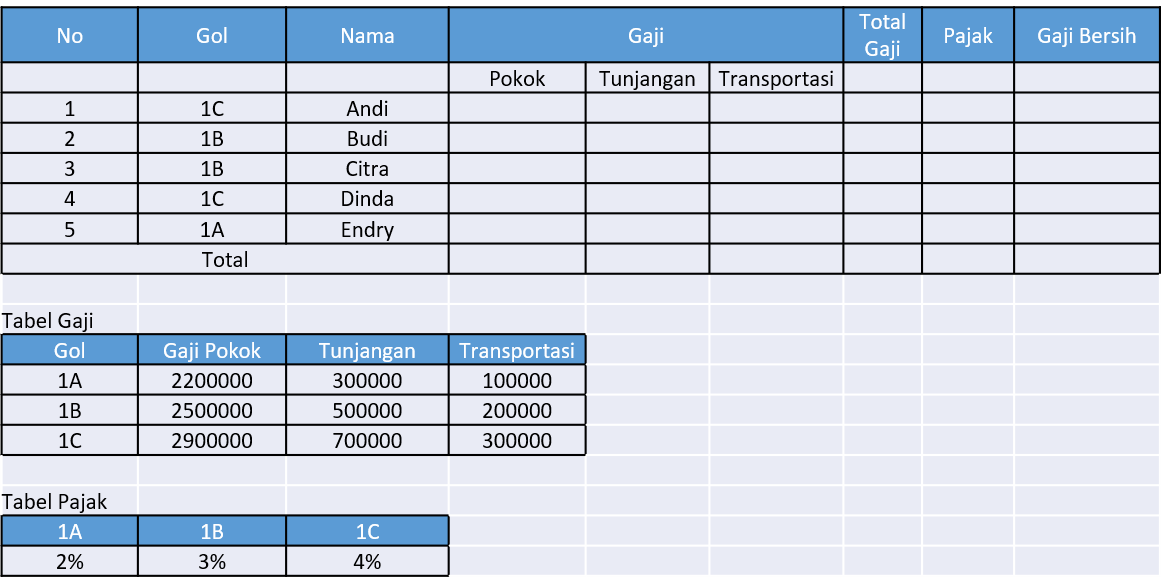
\includegraphics[width=1\linewidth]{images/tabel4} 

}

\caption{Gaji Karyawan Kopi Dari Hati}\label{fig:tabel4}
\end{figure}

\textbf{Keterangan:}

\begin{itemize}
\tightlist
\item
  Untuk gaji sesuai dengan gologan berdasarkan tabel gaji
\item
  Total Gaji =Gaji Pokok+Tunjangan+Transportasi
\item
  Pajak=Total Gaji x Pajak
\item
  Gaji Bersih= Total Gaji -- Pajak
\end{itemize}

\hypertarget{kasus-1.5}{%
\subsection*{Kasus 1.5}\label{kasus-1.5}}
\addcontentsline{toc}{subsection}{Kasus 1.5}

Pada bagian ini anda diharapkan untuk mampu menerapkan Fungsi IF Tunggal dan IF Majemuk untuk melengkapi Daftar Mahasiswa/i Manajemen Universitas Matana 2020 pada gambar \ref{fig:tabel5}.

\begin{figure}

{\centering 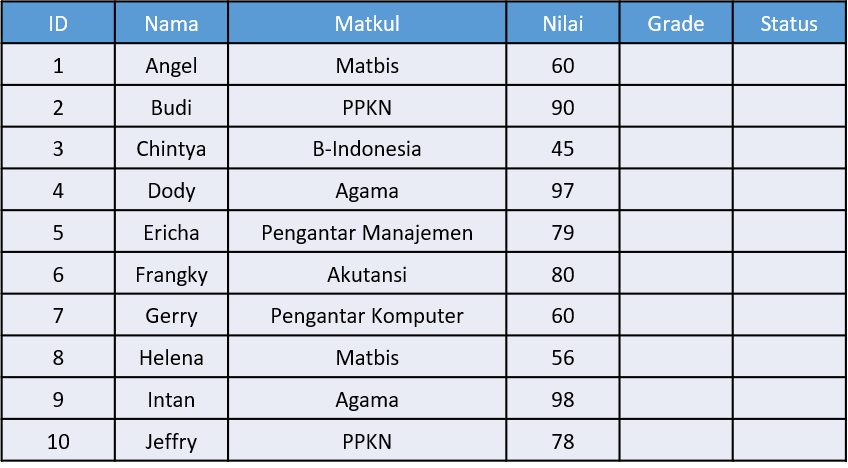
\includegraphics[width=1\linewidth]{images/tabel5} 

}

\caption{Daftar Mahasiswa/i}\label{fig:tabel5}
\end{figure}

\textbf{Keterangan:}

\begin{itemize}
\item
  Grade :

  \begin{itemize}
  \tightlist
  \item
    Grade A for Marks 90 -- 100,
  \item
    Grade B for marks 80 -- 89,
  \item
    Grade C for marks 70 -- 79,
  \item
    Grade D for marks 60 -- 69,
  \item
    Grade E for \textless{} 60
  \end{itemize}
\item
  Status :

  \begin{itemize}
  \tightlist
  \item
    if grade 75 is Complete,
  \item
    if grade \textless{} 75 is Failed
  \end{itemize}
\end{itemize}

\hypertarget{kasus-1.6}{%
\subsection*{Kasus 1.6}\label{kasus-1.6}}
\addcontentsline{toc}{subsection}{Kasus 1.6}

Selesaikan sistem persamaan linear dengan menggunakan Excel.

\hypertarget{Manajemen-Bisnis}{%
\chapter{Manajemen Bisnis}\label{Manajemen-Bisnis}}

\begin{center}\rule{0.5\linewidth}{0.5pt}\end{center}

Bab ini mencakup beberapa perhitungan matematika yang sering ditemukan dalam manajeman bisnis secara umum, dapat diterapkan diberbagai profesi bisnis seperti halnya Marketing (Pemasaran), Akuntansi, Produksi, Sumber Daya Manusia (HRD), Ekonomi, Keuangan, Analis Bisnis, dll. Dalam hal ini, saya mengasumsikan anda ingin menjadi owner/manajer perusahaan yang sukses, Anda perlu memahami beberapa hal mendasar dalam matematika bisnis seperti;

\hypertarget{rata-rata}{%
\section{Rata-rata}\label{rata-rata}}

Rata-rata nilai (besaran) yang diperoleh dari hasil jumlah tiap data dibagi dengan banyaknya data, nilai tersebut secara lumrah digunakan menjadi acuan untuk mewakili sekumpulan data. Pada saatnya nanti, ketika anda bekerja disuatu perusahaan, Manajer atau anda sendiri akan seringkali mempertanyakan, ``Berapa rata-rata penjualan perusahaan kita setiap Tahun,bulan, minggu, bahkan hingga harian''.

Perlu diketahui bahwa nilai rata-rata biasanya digunakan untuk mengevaluasi data sehingga lebih cepat dan menggambarkan seluruh data serta tidak dapat digunakan untuk menentukan nilai data tertentu di antara sekelompok data, sebagai contoh misalnya nilai rata-rata budi yaitu 85 jadi tidak bisa disimpulkan bahwa nilai untuk pelajaran Matematika Budi lebih dari 75. Nilai rata-rata tersebut bisa dipakai untuk membandingkan kelompok data yang satu dengan yang lainnya, seperti yg nilai rata-rata kelas yaitu 85 sedangkan nilai rata-rata kelas B yaitu 87 itu berarti kelas B lebih tinggi daripada kelas A.

Berikut rumus cara menghitung nilai rata-rata pada suatu kelompok,

\[ \small{ \text{Nilai Rata-rata}= {\text{Jumlah Nilai} \over \text{Banyak Data}} }\]

Berikut ini data nilai tes kuliah Matematika Bisnis 10 mahasiswa/i, kita akan menghitung nilai rata-rata yang diperoleh.

\begin{longtable}[]{@{}lcc@{}}
\toprule
No & Nama & Nilai\tabularnewline
\midrule
\endhead
1 & Eka Baper Sendiri & 85\tabularnewline
2 & Putri Woles Aja & 78\tabularnewline
3 & Bagus Sipemuja Mantan & 90\tabularnewline
4 & Neneng Gadis Desa & 75\tabularnewline
5 & Adi Korban Pelakor & 92\tabularnewline
6 & Bintang Bete & 85\tabularnewline
7 & Toni Raja Kepo & 85\tabularnewline
8 & Rina Capedeh & 82\tabularnewline
9 & Romy Kuper Abis & 96\tabularnewline
10 & Andika Pehape & 90\tabularnewline
\bottomrule
\end{longtable}

\[
\small{
\begin{aligned}
\text{Jumlah nilai} &= 85 + 78 + 90 + 75 + 92 + 85 + 85 + 82 + 96 + 90 = 858 \\
\text{Jumlah data} & = 10\\
\text{Nilai rata-rata} & = 858/10 = 85,8
\end{aligned}
}
\]

Jadi nilai rata-rata pelajaran Matematika 10 siswa tersebut adalah 85,8.

\hypertarget{nilai-rata-rata-dengan-penambahan-data}{%
\subsection{Nilai Rata-Rata dengan Penambahan Data}\label{nilai-rata-rata-dengan-penambahan-data}}

Apabila ada tambahan data maka jumlah nilai serta banyaknya data menjadi berubah. Jika ada penambahan satu data dengan nilai \(a\) maka,

\[
\small{
\begin{aligned}
\text{Jumlah nilai sekarang} &= \text{Jumlah nilai} + a \\ 
\text{Banyaknya data sekarang} & = \text{Banyaknya data} + 1 
\end{aligned}
}
\]

Contoh lainnya, misalkan ada penambahan dua data dengan nilai \(a_1\) dan \(a_2\) maka

\[
\small{
\begin{aligned}
\text{Jumlah nilai sekarang} & = \text{Jumlah nilai} + (a_1 + a_2) \\ 
\text{Banyaknya data sekarang} & = \text{Banyaknya data} + 2
\end{aligned}
}
\]

Sebagai contoh misalnya jika diketahui nilai rata-rata dari sekelompok data ditambah data tambahan. Misal diketahui nilai rata-rata tes mata pelajaran Bahasa Indonesia dari 8 orang Mahasiswa/i adalah 86.

Dua orang Mahasiswa/i tidak hadir saat tes dan mengikuti tes susulan, masing masing mendapat nilai 100 dan 87. Kita akan menghitung nilai rata-rata dari 10 orang Mahasiswa/i tersebut.

\[
\small{
\begin{aligned}
\text{Nilai rata-rata} & = \text{Jumlah nilai/banyaknya data} \\
\text{Jumlah nilai} & = \text{(Nilai rata-rata)} \times \text{(Banyaknya data)} \\
\text{Jumlah nilai} & = 86 \times 8 = 688 \\
\text{Jumlah nilai sekarang} & = 688 + 100 + 87 = 875 \\
\text{Banyaknya data sekarang} & = 8 + 2 = 10 \\
\text{Nilai rata-rata sekarang} &= 875 / 10 = 87,5
\end{aligned}
}
\]

Jadi nilai rata-rata pelajaran Bahasa Indonesia 10 Mahasiswa/i tersebut adalah 87,5.

\hypertarget{nilai-rata-rata-dengan-pengurangan-data}{%
\subsection{Nilai Rata-Rata dengan Pengurangan Data}\label{nilai-rata-rata-dengan-pengurangan-data}}

Jika ada pengurangan data maka jumlah nilai dan banyaknya data menjadi berubah. Jika ada pengurangan satu data dengan nilai \(a\) maka,

\[
\small{
\begin{aligned}
\text{Jumlah nilai sekarang}  & = \text{Jumlah nilai} – a\\
\text{Banyaknya data sekarang}& = \text{Banyaknya data} – 1
\end{aligned}
}
\]

Contoh lain, misalkan ada penguragan tiga data dengan nilai \(a_1 , a_2\) dan \(a_3\) maka,

\[
\small{
\begin{aligned}
\text{Jumlah nilai sekarang} &= \text{Jumlah nilai} – (a_1 + a_2 + a_3) \\
\text{Banyaknya data sekarang}& = \text{Banyaknya data} – 3
\end{aligned}
}
\]

\hypertarget{rasio}{%
\section{Rasio}\label{rasio}}

Rasio adalah suatu angka yang dibandingkan dengan angka lain sebagai suatu hubungan. Menurut Jonathan Golin, berpendapat bahwa rasio adalah suatu angka digambarkan dalam suatu pola yang dibandingkan dengan pola lainnya serta dinyatakan dalam persentase. Sedangkan keuangan adalah sesuatu yang berhubungan dengan akuntansi seperti pengelolaan keuangan dan laporan keuangan. Analisis rasio keuangan digunakan oleh dua pengguna utama, yakni investor dan manajemen. Investor menggunakan analisis rasio untuk melihat apakah perusahaan itu investasi yang bagus atau tidak.

Analisis Rasio Keuangan atau Financial Ratio adalah merupakan suatu alat analisis yang digunakan oleh perusahaan untuk menilai kinerja keuangan berdasarkan data perbandingan masing-masing pos yang terdapat di laporan keuangan seperti Laporan Neraca, Rugi /Laba, dan Arus Kas dalam periode tertentu.

\hypertarget{fungsi-analisis-rasio}{%
\subsection{Fungsi Analisis Rasio}\label{fungsi-analisis-rasio}}

\begin{itemize}
\tightlist
\item
  Rasio Likuiditas (Liquidity Ratio): Rasio likuiditas adalah rasio yang mengukur kemampuan likuiditas jangka pendek suatu perusahaan dengan melihat aktiva lancar perusahaan relatif terhadap hutang lancarnya.
\item
  Rasio Perputaran Persediaan (Inventory turnover ratio): Rasio perputaran persediaan mengukur aktivitas atau likuiditas perusahaan dilihat dari ketersediaan barang. Rasio ini menunjukkan efisiensi di mana perusahaan menggunakan seluruh aktivanya untuk menghasilkan penjualan.
\item
  Rasio Aktivitas (Activity Ratio): Rasio aktivitas menunjukkan tingkat efektivitas penggunaan aktiva atau kekayaan perusahaan kepada Anda.
\item
  Rasio Profitabilitas dan Rentabilitas (Profitability Ratio): Merupakan rasio yang menunjukkan tingkat imbalan atau perolehan dibanding penjualan atau aktiva.
\item
  Rasio Investasi (Investment Ratio): Rasio investasi merupakan rasio yang mengukur kemampuan perusahaan dalam memberikan kembalian atau imbalan kepada para pemberi dana, khususnya investor yang ada di pasar modal dalam jangka waktu tertentu.
\end{itemize}

\hypertarget{tujuan-analisis-rasio}{%
\subsection{Tujuan Analisis Rasio}\label{tujuan-analisis-rasio}}

\begin{itemize}
\tightlist
\item
  Sebagai alat barometer untuk melakukan forecasting atau memproyeksikan posisi keuangan dimasa yang akan datang.
\item
  Meninjau kondisi perusahaan saat ini, permasalahan dalam manajemen, operasional maupun, keuangan.
\item
  Alat ukur untuk melakukan efisiensi di semua departemen perusahaan.
\end{itemize}

\hypertarget{persen-perubahan}{%
\section{Persen Perubahan}\label{persen-perubahan}}

Dalam matematika, persentase perubahan digunakan untuk menunjukkan selisih atau perbedaan antara \textbf{nilai sebelum} dan \textbf{nilai sesudah} dalam bentuk persen nilai sebelum. Berikut adalah beberapa teknik yang digunakan untuk menganalisis persentasi perubahan yang sering ditemukan dalam laporan kinerja, perhitungan dalam keuangan, evaluasi laba atau rugi, dan juga sering digunakan untuk menganalisa kompetitor suatu perusahaan.

\hypertarget{analisis-tren}{%
\subsection{Analisis Tren}\label{analisis-tren}}

Analisa tren juga disebut analisis time-series. Analisis tren membantu manajer keuangan perusahaan menentukan bagaimana perusahaan cenderung melakukan kinerja dari waktu ke waktu. Analisis tren didasarkan pada data historis dari laporan keuangan perusahaan dan data perkiraan dari performa atau rencana ke depan perusahaan.

Salah satu cara yang populer dalam melakukan analisis tren adalah dengan menggunakan analisis rasio keuangan. Jika Anda menghitung rasio keuangan untuk perusahaan bisnis, Anda harus menghitung rasio minimal dua tahun terakhir, karena perbandingan rasio tidak berarti kecuali Anda memiliki sesuatu untuk membandingkannya dengan data tahun yang lain. Analisis tren akan lebih bagus lagi jika Anda memiliki dan menggunakan data rasio keuangan lebih dari 2 tahun.

\hypertarget{analisis-common-size}{%
\subsection{Analisis Common Size}\label{analisis-common-size}}

Analisis laporan keuangan common size menganalisis neraca dan laporan laba rugi dengan menggunakan persentase. Dalam analisis common size, semua akun laporan laba rugi dinyatakan sebagai persentase penjualan. Semua akun neraca dinyatakan sebagai persentase dari total aset. Misalnya, jika pada laporan laba rugi, setiap akun baris dibagi dengan penjualan, maka di neraca, setiap akun baris dibagi dengan total aset. Jenis analisis ini memungkinkan manajer keuangan untuk melihat laporan laba rugi dan neraca dalam format persentase yang mudah ditafsirkan, karena lebih mudah membuat perbandingan menggunakan persentase daripada angka absolut.

\hypertarget{analisis-persentase-perubahan}{%
\subsection{Analisis Persentase Perubahan}\label{analisis-persentase-perubahan}}

Analisis laporan keuangan ini sedikit lebih rumit. Bila menggunakan bentuk analisis ini, Anda harus menghitung tingkat pertumbuhan untuk semua akun laporan laba rugi dan akun neraca relatif terhadap tahun dasar. Teknik Ini adalah bentuk analisis laporan keuangan yang sangat kuat. Dengan teknik ini, Anda dapat melihat bagaimana berbagai akun laporan laba rugi dan akun neraca tumbuh atau relatif menurun terhadap pertumbuhan atau penurunan penjualan dan total aset.

\hypertarget{analisis-kempetitor}{%
\subsection{Analisis Kempetitor}\label{analisis-kempetitor}}

Analisis ini melibatkan perbandingan perusahaan dengan perusahaan lain di industri yang sama untuk melihat bagaimana perusahaan melakukan investasi secara finansial dibandingkan dengan industri lainnya. Jenis analisis ini sangat membantu manajer keuangan untuk melihat apakah ada penyesuaian finansial yang perlu dilakukan.

Teknik penghitungan rasio keuangan biasanya digunakan untuk analisis ini. Untuk melakukan pembandingan, Anda membutuhkan rasio rata-rata dari perusahaan lain di industri yang sama untuk dibandingkan dengan rasio bisnis Anda. Dengan teknik ini, Anda harus yakin bahwa rasio rata-rata industri lain tersebut telah dihitung dengan cara yang sama dengan rasio untuk perusahaan yang dihitung saat Anda melakukan analisis industri ini. Dengan menggunakan keempat teknik analisis laporan keuangan ini, seorang manajer keuangan akan mengetahui di mana potensi bisnis perusahaan baik secara finansial maupun internal berada, dibandingkan dengan perusahaan lain di industri yang sama.

\hypertarget{proporsi}{%
\section{Proporsi}\label{proporsi}}

Proporsi adalah pecahan yang pembilangnya merupakan bagian dari penyebutnya. Dengan kata lain persentase proporsi menghitung persentase dari sebuah variabel dengan membandingkan variabel tersebut dengan pembandingnya yang mana varibale tersebut merupakan bagian dari variable pembanding tersebut. Contohnya kasusnya begini: Pada acara pembukaan suatu Mall baru Jakarta, dilakukan pengumpulan data 2000 pengunnjung. Dari 2000 pengunjung tersebut 200 pengunjung ternyata adalah laki-laki dan sisanya adalah perempuan.

\begin{itemize}
\tightlist
\item
  Berapakah persentase pengunjung laki-laki dari seluruh pengunjung yang ada?
\item
  Berapakah persentase pengunjung perempuan dari seluruh pengunjung yang ada?
\end{itemize}

Untuk menghitung persentase tersebut mengikuti rumus matematika berikut:

\[ \% \text{ Proporsi}  = {\text{Nilai Proporsi} \over \text{Pembanding Proporsi}} \times 100 \%\]

\hypertarget{prorata}{%
\section{Prorata}\label{prorata}}

Pro rata adalah istilah Latin yang berarti ``dalam proporsi,'' mengacu pada alokasi proporsional atau distribusi atas sesuatu.

\hypertarget{memahami-prorata}{%
\subsection{Memahami Prorata}\label{memahami-prorata}}

Pro rata mengacu pada pembagian yang sama atas sesuatu -- termasuk suku bunga, pengeluaran, keuntungan pemegang saham (dividen), atau jumlah lain yang dibagi antara beberapa orang atau dalam kurun waktu tertentu. Istilah ini bisa digunakan di bidang apa saja, tetapi lebih sering muncul di bidang keuangan. Untuk menghitung bagian prorata, bagilah totalnya dengan jumlah unit yang ditentukan. Prorata sering digunakan secara bergantian dengan ``pembagian secara proporsional.''

\hypertarget{contoh-kasus-prorata}{%
\subsection{Contoh Kasus Prorata}\label{contoh-kasus-prorata}}

Katakanlah Perusahaan Ritel fiksi mengumumkan bahwa, pada kuartal keempat tahun ini, ia akan membayar dividen senilai Rp1 Miliar kepada pemegang saham. Setiap saham akan bernilai prorata, yang berarti jumlah proporsional dari dividen yang dibayarkan. Jika ada 500 saham yang beredar, jumlah prorata setiap saham bernilai Rp2,000,000 (Rp1 Miliar dibagi 500 saham).

Pro rata sering muncul dalam berbagai bidang, baik di bidang keuangan dan kehidupan sehari-hari. Istilah ini sering digunakan secara bergantian dengan ``pembagian secara proporsional,'' yang juga mengacu pada distribusi proporsional atas sesuatu, baik itu dividen, upah, atau suku bunga.Menetapkan pro rata hanya masalah membagi jumlah total sesuatu dengan jumlah bagian. Sebagai contoh sederhana, jika kamu memiliki total 100 unit sesuatu untuk dibagi menjadi 5 bagian yang sama, masing-masing bagian prorata adalah 20 unit (100 unit ÷ 5 bagian = 20 unit per bagian).

\hypertarget{kesimpulan-prorata}{%
\subsection{Kesimpulan Prorata}\label{kesimpulan-prorata}}

Seperti halnya membagi kue, jika anda mempunyai satu kue dan berencana membagikannya dengan lima temanmu, maka anda harus membagi kue menjadi enam. Bagian pro rata pencuci mulut setiap orang sama dengan seperenam kue.

\hypertarget{penerapan-prorata}{%
\subsection{Penerapan Prorata}\label{penerapan-prorata}}

Berikut adalah contoh beberapa hal di mana prorata sering muncul:

\hypertarget{a.-dividen-pemegang-saham-shareholder-dividends}{%
\subsubsection*{a. Dividen Pemegang Saham (Shareholder Dividends)}\label{a.-dividen-pemegang-saham-shareholder-dividends}}
\addcontentsline{toc}{subsubsection}{a. Dividen Pemegang Saham (Shareholder Dividends)}

Dalam dunia keuangan, pro rata sering digunakan untuk menentukan jumlah dividen yang akan diterima oleh pemegang saham. Ketika perusahaan telah membayar dividen, setiap pemegang saham akan menerima jumlah yang proporsional dengan persentase saham yang mereka miliki.Katakanlah ada total 500 saham di perusahaan, dan perusahaan membayar dividen senilai Rp500 juta. Dengan membagi jumlah total uang dan jumlah saham, bisa dipastikan bahwa setiap saham akan menghasilkan Rp1 juta dividen untukmu.

\hypertarget{b.-usaha-bersama-joint-ventures}{%
\subsubsection*{b. Usaha Bersama (Joint Ventures)}\label{b.-usaha-bersama-joint-ventures}}
\addcontentsline{toc}{subsubsection}{b. Usaha Bersama (Joint Ventures)}

Pro rata berperan penting dalam usaha bersama (ketika dua orang atau lebih memulai bisnis bersama). Usaha bersama termasuk perseroan terbatas, perusahaan, dan kemitraan. Seorang pemilik perusahaan menentukan bagiannya dari biaya dan laba. Berikut adalah contoh bagaimana prorata akan berperan dalam kasus kemitraan:

\begin{itemize}
\tightlist
\item
  \textbf{Tanggung Jawab:} Tingkat tanggung jawab mitra (biaya yang menjadi tanggung jawab mitra) dalam suatu bisnis ditentukan berdasarkan prorata yang sesuai dengan sahamnya di perusahaan. Katakanlah suatu kemitraan dituntut senilai Rp100 juta dan kalah. Mitra A memiliki 60\% saham di perusahaan, sementara Mitra B memiliki 40\%. Masing-masing tanggung jawab mitra sesuai dengan bagiannya di perusahaan. Mitra A bertanggungjawab atas 60\% dari utang (dalam hal ini, Rp60 juta), dan Mitra B bertanggungjawab atas 40\% (atau Rp40 juta).
\item
  \textbf{Keuntungan:} Sama halnya dengan tanggung jawab, bagian keuntungan pro rata dalam suatu kemitraan didasarkan pada bunga yang diperoleh perusahaan. Jika keuntungan dalam perusahaan yang sama mencapai Rp100 juta, Mitra A mendapat Rp60 juta dan Mitra B mendapat Rp40 juta.
\end{itemize}

\hypertarget{c.-suku-bunga-interest-rates}{%
\subsubsection*{c.~Suku Bunga (Interest Rates)}\label{c.-suku-bunga-interest-rates}}
\addcontentsline{toc}{subsubsection}{c.~Suku Bunga (Interest Rates)}

Pro rata bisa digunakan untuk membagi suku bunga menjadi bagian yang lebih kecil -- seringkali tarif tahunan menjadi tarif bulanan. Misalnya, jika suku bunga tahunan dalam pinjaman adalah 12\%, tingkat bulanannya adalah 1\% (12\% ÷ 12 bulan).

\hypertarget{d.-surat-perjanjian-asuransi-insurance-policies}{%
\subsubsection*{d.~Surat Perjanjian Asuransi (Insurance Policies)}\label{d.-surat-perjanjian-asuransi-insurance-policies}}
\addcontentsline{toc}{subsubsection}{d.~Surat Perjanjian Asuransi (Insurance Policies)}

Prorata ikut berperan ketika kamu membatalkan surat perjanjian asuransi lebih awal. Jika kamu membayar Rp6 juta untuk asuransi selama enam bulan dan dibatalkan setelah tiga bulan, perusahaan asuransi akan mengembalikan jumlah yang setara. Dalam hal ini, karena kamu membatalkan kebijakan, kamu akan memenuhi syarat utuk pengembalian uang senilai 50\%. Pro rata juga digunakan untuk menentukan pembayaran bulanan kamu. Seringkali perusahaan asuransi menetapkan harga suatu kebijakan selama periode enam atau 12 bulan, tetapi banyak pelanggan yang tidak mau membayar bunga mereka sekaligus. Sebaliknya, perusahaan asuransi membagikan bunga sehingga pelanggan membayar jumlah yang ditentukan setiap bulan.

\hypertarget{e.-pembayaran-pinjaman-loan-payments}{%
\subsubsection*{e. Pembayaran Pinjaman (Loan Payments)}\label{e.-pembayaran-pinjaman-loan-payments}}
\addcontentsline{toc}{subsubsection}{e. Pembayaran Pinjaman (Loan Payments)}

Contoh pro rata lainnya adalah bagian pinjaman menjadi pembayaran bulanan. Saat kamu mengambil pinjaman -- baik itu pinjaman pribadi, pinjaman mobil, atau hipotek -- saldo dibagi selama masa pinjaman. Dalam gabungan bunga, adalah bagaimana pemberi pinjaman menentukan seperti apa cara pembayaran bulanannya.

\hypertarget{f.-apartemen}{%
\subsubsection*{f.~Apartemen}\label{f.-apartemen}}
\addcontentsline{toc}{subsubsection}{f.~Apartemen}

Pro rata sering muncul dalam penyewaan apartemen. Umumnya, sewa dikenakan biaya bulanan, tetapi bagaimana jika kamu tidak tinggal di apartemen selama sebulan penuh? Mungkin kamu mulai menyewa beberapa hari dalam sebulan atau berakhir di pertengahan bulan.Dalam hal ini, pemilik apartemen mungkin akan membuat prorata sewa kamu, atau hanya menagih berdasarkan jumlah hari yang kamu habiskan di apartemen. Sebagai contoh, katakanlah sewa bulanan kamu adalah Rp5 juta, dan kamu mulai menyewa pada 3 September. Pemilik apartemen akan menghitung jumlah pro rata yang kamu miliki dengan menentukan biaya sewa harian dan mengalikannya dengan jumlah hari kamu saat berada di Apartemen.Sejak September ada 30 hari, pemilik akan membagi Rp5 juta dengan 30 untuk menentukan tarif harian, hasilnya adalah Rp166 ribu. Kemudian, dia akan mengalikan tarif harian dengan jumlah hari yang dihabiskan di apartemen, atau Rp166 x 28 hari. Jadi, total biaya akhir Rp4,648,000.

\hypertarget{g.-gaji-pro-rata}{%
\subsubsection*{g. Gaji Pro Rata}\label{g.-gaji-pro-rata}}
\addcontentsline{toc}{subsubsection}{g. Gaji Pro Rata}

Salah satu kegunaan pro rata pada umumnya berlaku untuk karyawan yang memiliki gaji. Umumnya, gaji adalah upah yang dinyatakan sebagai jumlah tahunan, bukan gaji per jam. Gaji biasanya mengasumsikan karyawan yang bekerja tahunan dengan jumlah minimum jam per minggu (biasanya 40).Jika kamu seorang karyawan yang mendapatkan gaji tahunan, prorata digunakan untuk menentukan berapa banyak gaji yang kamu dapatkan. Misalnya, katakanlah kamu mendapatkan gaji tahunan Rp120 juta dan dibayar setiap dua minggu. Kamu akan digaji 26 kali dalam setahun, sehingga pemberi kerja akan menjumlah gaji dan dibagi 26 untuk menentukan berapa yang harus dibayarkan padamu setiap dua minggu. Hasil gaji selama dua minggu adalah Rp4,615,000.

\hypertarget{latihan}{%
\section{Latihan}\label{latihan}}

Untuk memastikan anda memahami materi dengan baik, berikut ini diberikan latihan yang mencakup pembahasan diatas secara praktikal dalam Excel. Silahkan download file latihan \href{https://github.com/Bakti-Siregar/Matematika-Bisnis/blob/master/data/matematika-manajemen-bisnis.xlsx?raw=true}{disini}.

  \bibliography{book.bib,packages.bib}

\end{document}
